
% This LaTeX was auto-generated from an M-file by MATLAB.
% To make changes, update the M-file and republish this document.

\documentclass{article}
\usepackage{graphicx}
\usepackage{color}
\usepackage{listings}
\usepackage[framed]{mcode}
\usepackage{fullpage}
\usepackage{amsmath}
\usepackage[utf8x]{inputenc}
\usepackage{import}
\usepackage{setspace}
\usepackage{hyperref}
\definecolor{lightgray}{gray}{0.5}
\setlength{\parindent}{0pt}

\begin{document}

    
    
%\section*{}


\title{BE 521: Homework 1 \\{\normalsize Exploring Neural Signals} \\{\normalsize Spring 2021}}
\author{33 points}
\date{Due: Tuesday 2/2/2021 10 PM}
\maketitle
\textbf{Objective:} Working with the IEEG Portal to explore different Neural signals


\begin{center}
\author{Jal Mahendra Panchal}
\end{center}


\section{Seizure Activity (16 pts)}
The dataset \texttt{I521\_A0001\_D002} contains an example of human intracranial EEG (iEEG) data displaying seizure activity. It is recorded from a single channel (2 electrode contacts) implanted in the hippocampus of a patient with temporal lobe epilepsy being evaluated for surgery. In these patients, brain tissue where seizures are seen is often resected. You will do multiple comparisons with this iEEG data and the unit activity that you worked with in Homework 0 \texttt{(I521\_A0001\_D001)}. You will have to refer to that homework and/or dataset for these questions.
\begin{enumerate}
 \item Retrieve the dataset in MATLAB using the IEEGToolbox and generate a \emph{session} variable as before (No need to report the output this time). What is the sampling rate of this data? What is the maximum frequency of the signal content that we can resolve? (2 pts)

\begin{lstlisting}
%Adding workspace path
addpath(genpath('/Users/jalpanchal/git/be521'));

%create session
% dataset I521_A0001_D002.
session_sez = IEEGSession('I521_A0001_D002', 'jalpanchal', 'jal_ieeglogin.bin');

%Calculate sampling frequency in Hz
sampling_frequency_hz = session_sez.data.sampleRate

%Maximum resolvable frequency = sampling frequncy/2.
max_resolvable_freq = sampling_frequency_hz/2
\end{lstlisting}

\color{lightgray} \begin{lstlisting}IEEGSETUP: Adding 'ieeg-matlab.jar' to dynamic classpath
IEEGSETUP: Found log4j on Java classpath.
URL: https://www.ieeg.org/services
Client user: jalpanchal
Client password: ****

sampling_frequency_hz =

   200


max_resolvable_freq =

   100

\end{lstlisting} \color{black}

 \item How does the duration of this recording compare with the recording from HW0 \texttt{(I521\_A0001\_D001)}? (2 pts)

\begin{lstlisting}
duration_in_usec = session_sez.data(1).rawChannels(1).get_tsdetails.getDuration;
duration_in_sec = duration_in_usec/1e6

disp("This resording has a duration of 644.995s as compared to 10s for I521_A0001_D001")
\end{lstlisting}

\color{lightgray} \begin{lstlisting}
duration_in_sec =

  644.9950

This resording has a duration of 644.995s as compared to 10s for I521_A0001_D001
\end{lstlisting} \color{black}

 \item Using the time-series visualization functionality of the IEEG Portal, provide a screenshot of the first 500 ms of data from this recording. (2 pts)

Include screenshot:
\begin{lstlisting}
%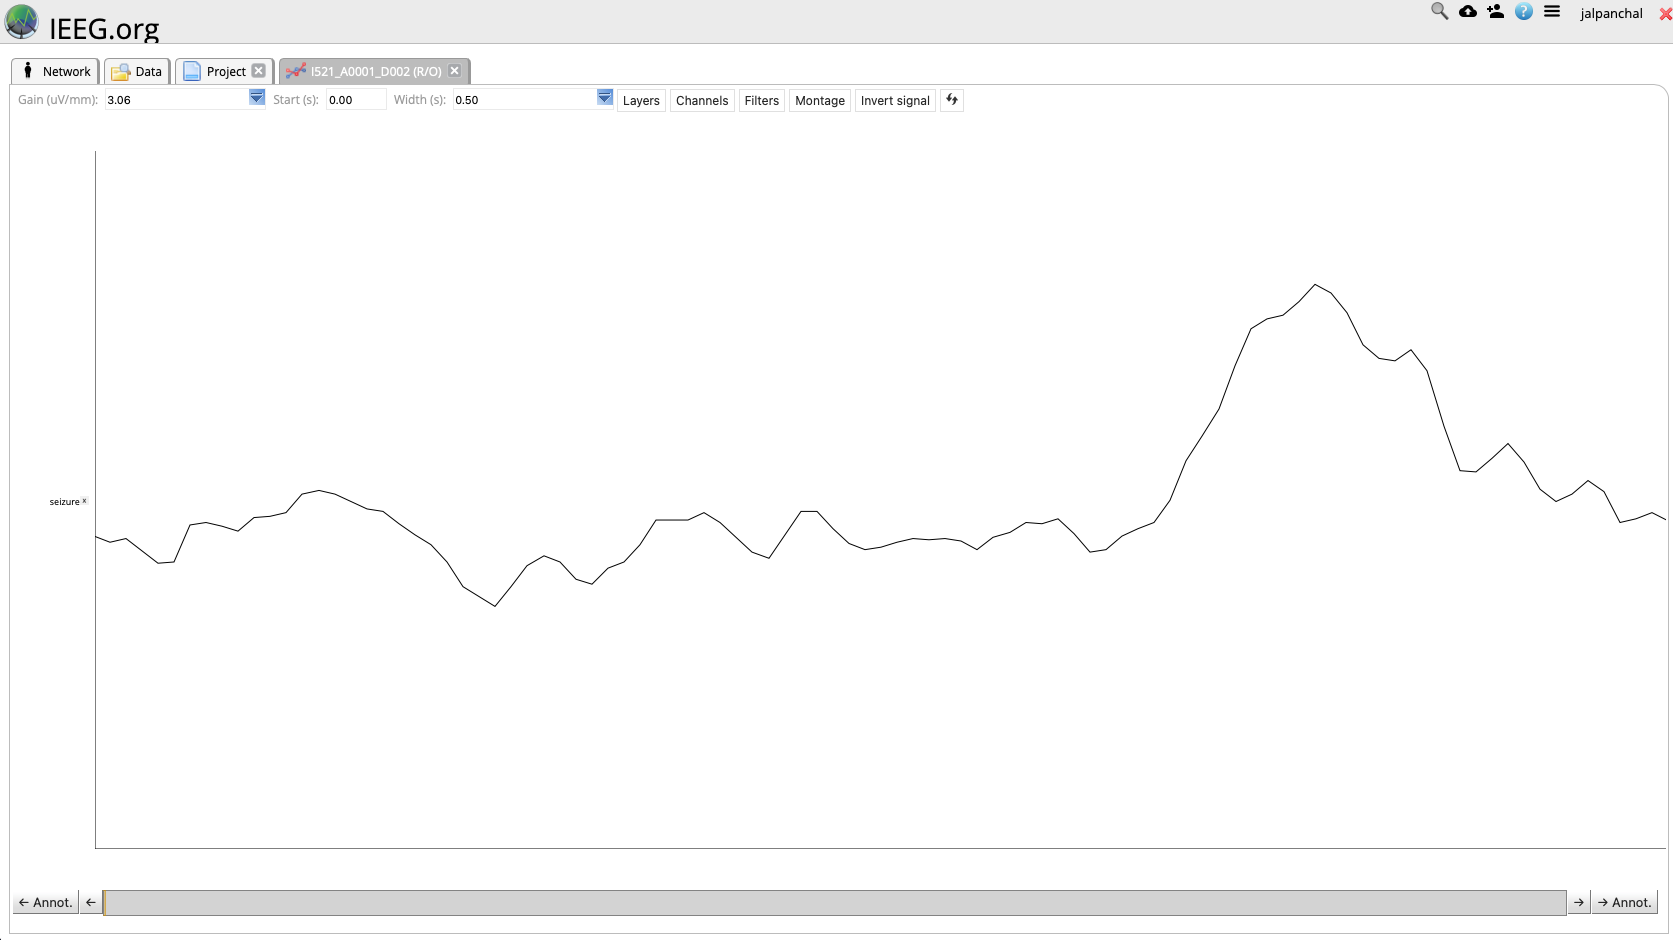
\includegraphics[scale=0.25]{screenshot_q3_hw1.png}\\
\end{lstlisting}

 \item Compare the activity in this sample with the data from HW0.  What differences do you notice in the amplitude and frequency characteristics? (2 pts)


\begin{enumerate}
  \item The signal in I521_A0001_D002 has higher signal amplitude (Close
  to peak-peak amplitude of 4500 uV) while the I521_A0001_D001 signal has a
  much lower signal amplitude of about 180 uV peak-peak.
  \item The

\begin{lstlisting}
%To plot frequency spectrum of each of the signals
%I521_A0001_D002

fs = sampling_frequency_hz
len = duration_in_sec
t = 0:1/fs:len-1/fs;
x = session_sez.data.getvalues(1, len * 1e6, 1);
y = fft(x);
n = length (x);
f = (0:n-1)*(fs/n);
power = abs(y).^2/n;

figure();
subplot(3,2,3);
plot(f(1:floor(n/2)),power(1:floor(n/2)))
title('Power Spectrum - I521\_A0001\_D002')
xlabel('Frequency (Hz)')
ylabel('Power (\mu V^2)')

%Plot of signal in time domain
subplot(3,2,1);
plot(t, x);
ylabel('Amplitude (\mu V)');
xlabel('Time (sec)');
title('Multi-unit signal - I521\_A0001\_D002');

%plotting a spectogram
subplot(3,2,5);
[p,f,t] = pspectrum(x,fs,'spectrogram');
waterfall(f,t,p');
xlabel('Frequency (Hz)')
ylabel('Time (seconds)')
zlabel('Normalized Power (\mu V^2)')
title('Spectogram - I521\_A0001\_D002');
wtf = gca;
wtf.XDir = 'reverse';
view([30 45])


%I521_A0001_D001

%Plot of Power Spectrum
session_1 = IEEGSession('I521_A0001_D001', 'jalpanchal', 'jal_ieeglogin.bin');
sampling_frequency_hz_1 = session_1.data.sampleRate
duration_in_sec_1 = session_1.data(1).rawChannels(1).get_tsdetails.getDuration/1e6;

fs = sampling_frequency_hz_1
len = duration_in_sec_1
t = 0:1/fs:len-1/fs;
x = session_1.data.getvalues(1, len * 1e6, 1);
y = fft(x);
n = length (x);
f = (0:n-1)*(fs/n);
power = abs(y).^2/n;

%Plotting power spectrum
subplot(3,2,4);
plot(f(1:floor(n/2)),power(1:floor(n/2)))
title('Power Spectrum - I521\_A0001\_D001')
xlabel('Frequency (Hz)')
ylabel('Power (\mu V^2)')

%Plot of signal in time domain
subplot(3,2,2);
plot(t, x);
ylabel('Amplitude (\mu V)');
xlabel('Time (sec)');
title('Multi-unit signal - I521\_A0001\_D001');

%plotting a spectogram
subplot(3,2,6);
[p,f,t] = pspectrum(x,fs,'spectrogram');
waterfall(f,t,p');
xlabel('Frequency (Hz)')
ylabel('Time (seconds)')
zlabel('Normalized Power (\mu V^2)')
title('Spectogram - I521\_A0001\_D001');
wtf = gca;
wtf.XDir = 'reverse';
view([30 45])
\end{lstlisting}

\color{lightgray} \begin{lstlisting}
fs =

   200


len =

  644.9950

IEEGSETUP: Adding 'ieeg-matlab.jar' to dynamic classpath
Warning: Objects of edu/upenn/cis/db/mefview/services/TimeSeriesDetails
class exist - not clearing java 
Warning: Objects of edu/upenn/cis/db/mefview/services/TimeSeriesInterface
class exist - not clearing java 
IEEGSETUP: Found log4j on Java classpath.
URL: https://www.ieeg.org/services
Client user: jalpanchal
Client password: ****

sampling_frequency_hz_1 =

       32051


fs =

       32051


len =

    10

\end{lstlisting} \color{black}


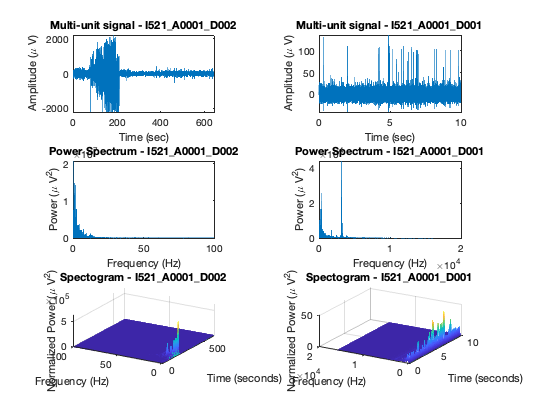
\includegraphics [width=5in]{HW1_Questions_01.png}

 \item The unit activity sample in \texttt{(I521\_A0001\_D001)} was high-pass filtered to remove low-frequency content. Assume that the seizure activity in \texttt{(I521\_A0001\_D002)} has not been high-pass filtered. Given that the power of a frequency band scales roughly as $1/f$, how might these differences in preprocessing contribute to the differences you noted in the previous question? (There is no need to get into specific calculations here. We just want general ideas.) (3 pts)


 \item Two common methods of human iEEG are known as electrocorticography (ECoG) and stereoelectroencephalography (SEEG). For either of these paradigms (please indicate which you choose), find and report at least two of the following electrode characteristics: shape, material, size. Please note that exact numbers aren't required, and please cite any sources used. (3 pts)


 \item What is a local field potential? How might the  characteristics of human iEEG electrodes cause them to record local field potentials as opposed to multiunit activity, which was the signal featured in HW0 as recorded from 40 micron Pt-Ir microwire electrodes? (2 pts)


\end{enumerate}


\section{Evoked Potentials (17 pts)}
The data in \texttt{I521\_A0001\_D003} contains an example of a very common type of experiment and neuronal signal, the evoked potential (EP). The data show the response of the whisker barrel cortex region of rat brain to an air puff stimulation of the whiskers. The \texttt{stim} channel shows the stimulation pattern, where the falling edge of the stimulus indicates the start of the air puff, and the rising edge indicates the end. The \texttt{ep} channel shows the corresponding evoked potential.
Once again, play around with the data on the IEEG Portal, in particular paying attention to the effects of stimulation on EPs. You should observe the data with window widths of 60 secs as well as 1 sec. Again, be sure to explore the signal gain to get a more accurate picture. Finally, get a sense for how long the trials are (a constant duration) and how long the entire set of stimuli and responses are.


\begin{enumerate}
 \item Based on your observations, should we use all of the data or omit some of it? (There's no right answer, here, just make your case either way in a few sentences.) (2 pts)


 \item Retrieve the \texttt{ep} and \texttt{stim} channel data in MATLAB. What is the average latency (in ms) of the peak response to the stimulus onset over all trials? (Assume stimuli occurs at exactly 1 second intervals)(3 pts)


 \item In neuroscience, we often need to isolate a small neural signal buried under an appreciable amount of noise.  One technique to accomplish this is called the spike triggered average, sometimes called signal averaging. This technique assumes that the neural response to a repetitive stimulus is constant (or nearly so), while the noise fluctuates from trial to trial - therefore averaging the evoked response over many trials will isolate the signal and average out the noise.
 Construct a spike triggered average plot for the data in \texttt{I521\_A0001\_D003}.  Plot the average EP in red.  Using the commands \texttt{hold on} and \texttt{hold off} as well as \texttt{errorbar} and \texttt{plot}, overlay error bars at each time point on the plot to indicate the standard deviation of the responses at any given time point.  Plot the standard deviation error bars in gray (RGB value: [0.7 0.7 0.7]). Make sure to give a proper legend along with your labels. (4 pts)


 \item
  \begin{enumerate}
	\item We often want to get a sense for the amplitude of the noise in a single trial. Propose a method to do this (there are a few reasonably simple methods, so no need to get too complicated). Note: do not assume that the signal averaged EP is the ``true'' signal and just subtract it from that of each trial, because whatever method you propose should be able to work on the signal from a single trial or from the average of the trials. (4 pts)


	\item Show with a few of the EPs (plots and/or otherwise) that your method gives reasonable results. (1 pt)


	\item
    \begin{enumerate}
        \item Apply your method on each individual trial and report the mean noise amplitude across all trials. (1 pt)


        \item Apply your method on the signal averaged EP and report its noise. (1 pt)


	    \item Do these two values make sense? Explain. (1 pt)


    \end{enumerate}
  \end{enumerate}
\end{enumerate}




\end{document}
    
